\phantomsection

\numberedsection{RF6.4 Borrar Atributo}

\subsection*{Descripción}
Los usuarios pueden borrar los atributos de usuario ya existentes en la cuenta.
\vspace{0.15cm}

\textbf{Pre-condición}\par
El usuario ha iniciado sesión en su cuenta en Mini PIM, tiene acceso a la sección de gestión de atributos y hay al menos un atributo de usuario creado.\par
\vspace{0.15cm}

\textbf{Post-condición}
\begin{itemize}
    \item Caso de éxito: El atributo es borrado y eliminado de la base de datos
    \item Caso mínimo: El sistema notifica al usuario el resultado de la acción borrar atributo; exitosa o fallida.
\end{itemize}

\textbf{Prioridad: }
Alta
\vspace{0.15cm}

\textbf{Autor(es): }
Pablo Ortega\par
\vspace{0.15cm}

\textbf{Control de cambios: }
\begin{itemize}
    \item Versión 1: Definición del caso de uso.
\end{itemize}

\numberedsubsection{Escenario principal}
\begin{enumerate}
    \item El usuario selecciona el atributo que quiere modificar.
    \item El usuario pulsa el botón de borrar.
    \item El sistema borra el atributo.
    \item El sistema muestra al usuario un mensaje confirmando que el atributo ha sido borrado con éxito.
\end{enumerate}

\numberedsubsection{Escenarios alternativos}

\numberedsubsection{Casos de Prueba}
\underline{Escenario: Principal}\par
\vspace{0.15cm}
\textbf{Dado} que el usuario ha iniciado sesión en su cuenta en Mini PIM,\par
\textbf{Y} se encuentra en la sección de atributos,\par
\textbf{Y} selecciona un atributo,
\textbf{Cuando} pulsa el botón de borrar,\par
\textbf{Entonces} el sistema borra el atributo de la base de datos y vuelve a mostrar la lista de atributos.\par
\vspace{0.20cm}

\numberedsubsection{Bocetos}
\begin{figure}[H]
    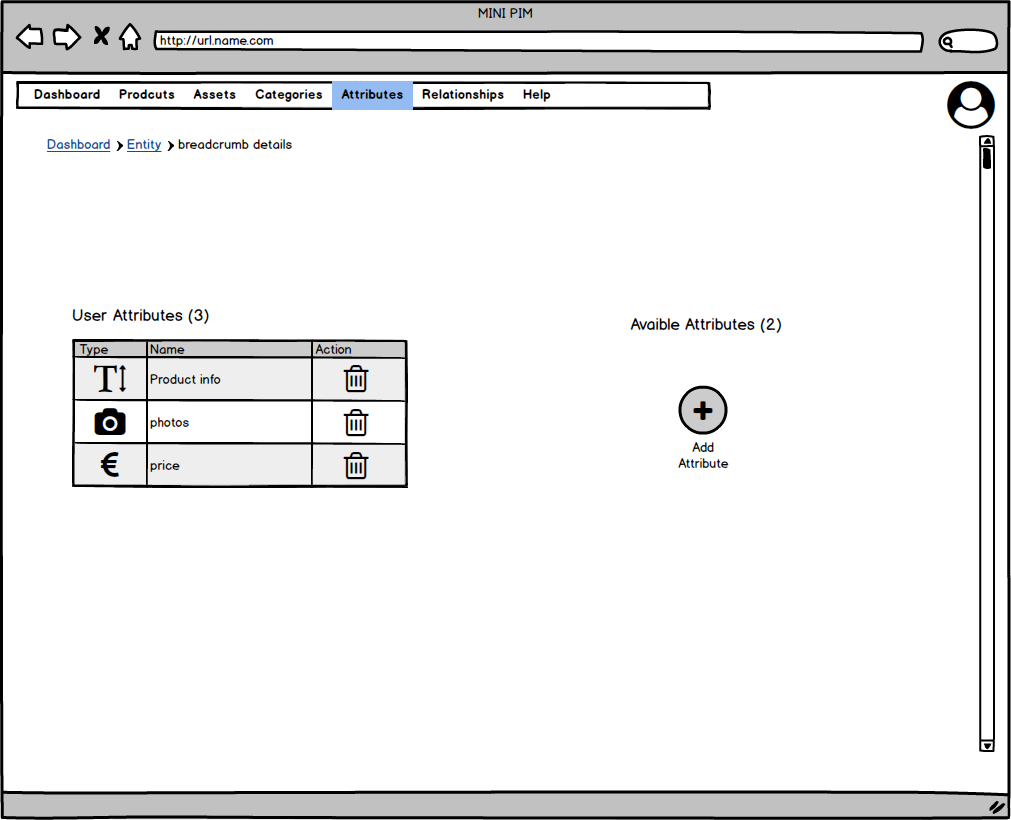
\includegraphics[width=1\linewidth]{mockups/RF6.2Leer_Atributo.png}
    \caption{Apartado Productos}
   \end{figure}
\vspace{1.0cm}

\begin{figure}[H]
    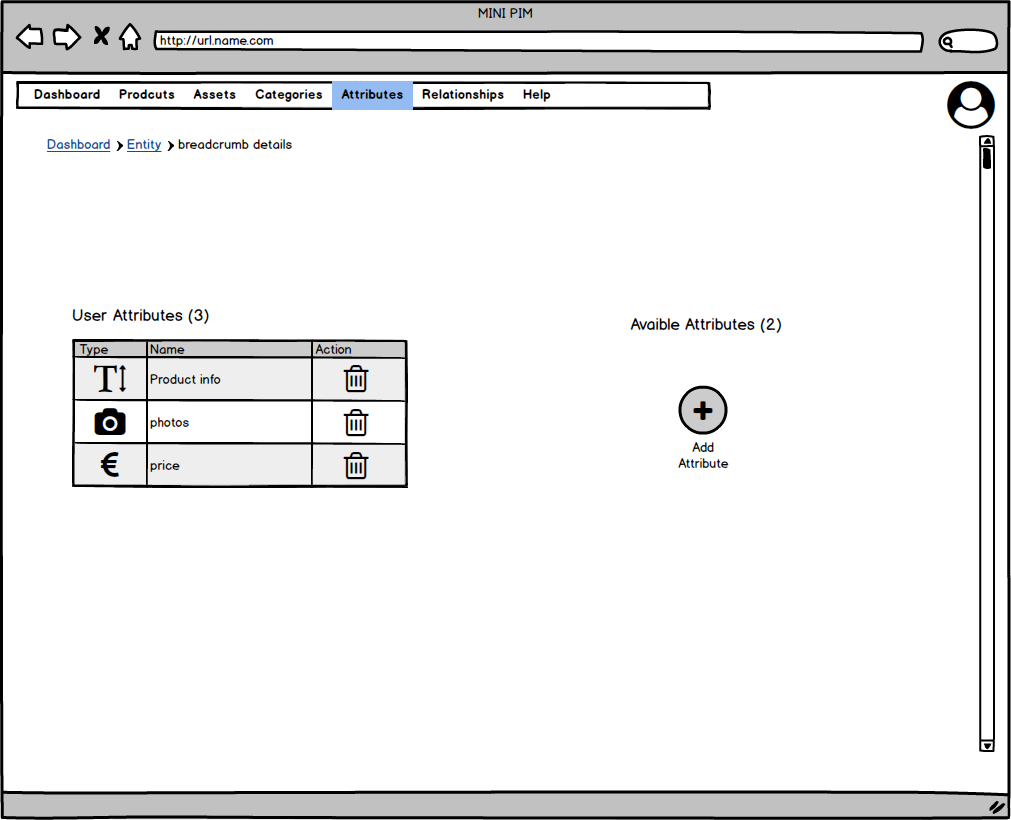
\includegraphics[width=1\linewidth]{mockups/RF6.2Leer_Atributo.png}
    \caption{Menú de creación}
   \end{figure}
\vspace{1.0cm}

\newpage %Inicia en una nueva página otro caso de uso